\documentclass[conference]{IEEEtran}

\usepackage{algorithmic}
\usepackage{amsfonts, amsmath, amsthm}
\usepackage{array}
\usepackage{bm}
\usepackage{booktabs}
\usepackage{caption}
\usepackage{cite}
\usepackage{fullpage}
\usepackage{gensymb}
\usepackage{geometry}
\usepackage{graphicx}
\usepackage{listings}
\usepackage{mathtools}
\usepackage{pifont}
\usepackage{textcomp}
\usepackage{tikz}
\usepackage{tkz-graph}
\usepackage{verbatim}
\usepackage{xcolor}

\usetikzlibrary{shapes.geometric}

\def\BibTeX{{\rm B\kern-.05em{\sc i\kern-.025em b}\kern-.08em
    T\kern-.1667em\lower.7ex\hbox{E}\kern-.125emX}}

\newcolumntype{L}{>{$}l<{$}} % math-mode version of "l" column type

\makeatletter
\newcommand\mathboxed[1]{%
    \mathpalette\@mathboxed{#1}%
}
\newcommand\@mathboxed[2]{%
    \tikz[baseline=(math.base),outer sep=auto]{\node[draw,rectangle,inner
    sep=2.8pt]
    (math) {$#1#2$};
    \path (math.north)--++(0,1pt);
    \path (math.south)--++(0,-1pt);}%
}
\makeatother

\begin{document}
\title{%
  CENG435 Term Project: Part Two \\
  \large Transferring a large file over an unreliable network}

\author{
    \IEEEauthorblockN{Narmin Aliyeva}
    \IEEEauthorblockA{}
\and
    \IEEEauthorblockN{Berk Ozbalci}
    \IEEEauthorblockA{}
}

\maketitle

\section{Introduction}
In the part two of our term project, we are asked to develop a reliable data transfer protocol
over UDP, that supports pipelining and multi-homing. There are a total of two experiments that
was conducted over our newly-developed protocol. In the first experiment, we measured the time
taken to transfer a file from the source host to the destination host over a single router. In
the second experiment, we do the same thing, but except this time we route the packets over two
routers in the same time; where the protocol has to dynamically change routing strategies
depending on link failures (i.e. if one of the routers are down, it must fall back to delivering
files over a single router).

\section{Design and Implementation}
Python 3.6.5, the version which was installed in GENI VMs, was used throughout the project.

For maintaining nodes (i.e. configuring emulated losses using NetEm, updating scripts, running
experiments and collecting data) an array of Bash scripts were developed.

We created a monolithic Python module and deployed it to all nodes. Every node receives the same
copy of the module, only differing in the way they run the modules, i.e. running the script with
\textbf{--router} will set the current node as a router.


\subsection{Protocol Design}
We used the Go-Back-N ARQ\footnote{Automatic repeat request} protocol for achieving reliable data transfer.

% TODO Maybe explain GBN here?

\subsubsection{Packet Structure}

Our packet structure is quite simple. It is layed out as follows:

\begin{itemize}
    \item \textbf{Byte 0:} Contains a boolean value representing whether this packet is an ACK
    (acknowledgement) or not. This never had any practical value in our experiments, but we added
    it to future-proof our protocol.
    \item \textbf{Byte 1:} Contains a boolean value representing whether this packet is the final
    packet or not. This is used to terminate the source and destination processes when the entire
    file has been transmitted, which is one of the requirements imposed on the experiment software.
    \item \textbf{Bytes 2-5:} Contains an unsigned 4-byte integer that represents the sequence number
    of this packet. Sequence numbers do not have any special meaning in this implementation, they are
    just the same as sequence numbers in the generic Go-Back-N ARQ protocol.
    \item \textbf{Bytes 6-10:} Contains an unsigned 4-byte integer that represents the length of the
    payload (in number of bytes).
    \item \textbf{Bytes 11-969:} The payload. The maximum payload size is 958 bytes, because the
    header takes up 10 bytes and the footer (checksum) takes up 32 bytes. The maximum allowed packet
    size is 1000, and we figured that having a larger packet size would benefit the time taken to
    deliver files, so we fill the rest of the given space with the payload.
    \item \textbf{Bytes 969-1000:} The MD5 hash of the packet, used as a checksum.
    This is always 32 bytes long.
\end{itemize}

In our implementation, checksum failure will immediately cause the program to exit with an exception.
While it is trivial to refactor the code so that checksum failures will cause the source to retransmit,
we decided to leave it as-is, so as to help debugging the problem if anything goes wrong.

\subsubsection{Application-Layer Routing}
Our implementation does not have much "routing". In both experiment one and experiment two, the
source node decides which router to send a packet to.

The nodes \textbf{r1}, \textbf{r2}, \textbf{r3} are always operating in the same mode: if a packet
arrives from the source node, it is forwarded to the destination node. If a packet arives from the
destination node, it is forwarded to the source node.

In both experiments, the destination node sends ACKs to the same address the packet is coming from. So
the same router that was used to send a packet will be used to send that packet's acknowledgement. This
fits the criteria for both experiments.

In the event of a link failure, a scenario may occur where the acknowledgement from the destination
node cannot be transmitted to the source node over the same link, because it was shut down after
transmitting the packet to the destination node. That scenario would not be problematic in our
design, because it will be the same thing as an ACK getting dropped on the way, meaning that the
sender will have the chance to consider using a different router.

There is a port number convention (the same used in the Term Project part one) that helped us in
conceptualizing connections and links.

% TODO Explain this as well?

\section{Experiment Results}

In this section, we will present the experiment results and discuss the effects of packet loss
on file transfer time. In general, a higher loss results in a greater file transfer time. First,
we shall try to come up with a theoretical expected relation using probability and mathematics.

\subsection{Theoretical Expectation}

Losing packets with probability $p$ over each link means that the packet will be transmitted
successfully with $1 - p$. This does not mean, however, the source will successfully transmit
approximately $(1-p) \times N$ packets, where $N$ is the total intended number of packets. We
need to calculate the "effective loss", that is the cumulative effect of packets being subjected
to loss from one end to another, and back again.

For experiment 1, every packet is routed from \textbf{s} to \textbf{r3}, then to \textbf{d}, and
back again. This results in 4 transmissions, and therefore 4 instances where packet loss could
potentially occur. The $1-p$ probability applies four times, so the total probability is
$(1-p)^4$.

\textbf{Note.} In practice, more complicated networks with different link structures and more
complicated loss parameters associated with them, modeling them with Markov chains will yield
a better result. This would be required for Experiment 2, but we're making this calculation only
for Experiment 1.

For the given loss values, the below table shows the computed values:

\begin{table}[h]
    \centering
    \renewcommand{\arraystretch}{2.5}
        \begin{tabular}{|c|c|c|c|}
        \hline
                            & Case I & Case II & Case III \\
        \hline
                $p$         & 0.050  & 0.150   & 0.380    \\
        \hline
                $1-p$       & 0.950  & 0.850   & 0.620    \\
        \hline
                $(1-p)^4$   & 0.814  & 0.522   & 0.147    \\
        \hline
                $m/(1-p)^4$ & 1.000  & 1.560   & 5.512    \\
        \hline
        \end{tabular}
    \caption{Effective packet loss}
    \label{table:theoretical}
\end{table}

The final row represents the \textit{effective packet loss time penalty factor}, which is the
multiplicative inverse of the penultimate row, normalized with respect to Case I. This means that
if sending the file in Case I takes 1 minute, sending the file in Case II will take at least
1.56 minutes. We say \textit{at least} because there are some other factors that aren't taken into
account:

\begin{itemize}
    \item The emulated loss is not exact. We observed that even without setting any NetEm losses,
    there was a certain amount of packet loss.
    \item The processing-time of our scripts may not be scaling linearly. We made our best efforts
    to ensure that everything will scale linearly, but there may be oversights.
\end{itemize}

With the theoretical expectations defined, we can now move on to the experimental results.

\subsection{Caveat}
Since we didn't have enough time to collect enough data to achieve a the desired margin of error
(2.5\%), we significantly relaxed the margin of error to 10\%. Furthermore, we did the confidence
interval computation for only the first case of Experiment 1. The rest of the experiment cases
were not repeated more than 5 times.

\subsection{Experiment 1}

\begin{figure}
    \center
    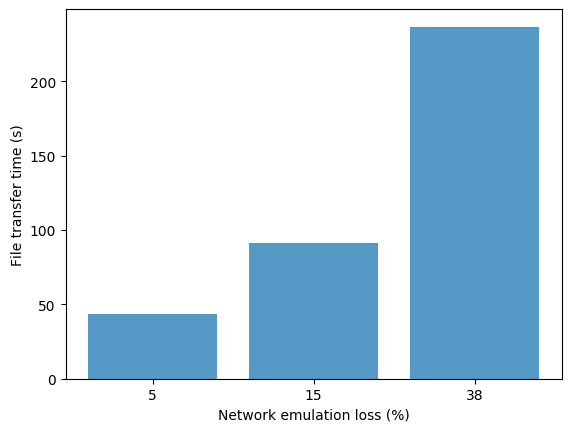
\includegraphics[width=\columnwidth]{images/chart}
    \caption{Packet loss vs. file transfer time}
    \label{fig:graphexp1}
\end{figure}

In the table below, you can see the experimental results obtained. CI stands for Confidence Interval,
and $N$ is the number of samples obtained to retrieve the results.

\begin{table}[h]
    \centering
    \renewcommand{\arraystretch}{2.5}
        \begin{tabular}{|c|c|c|c|}
        \hline
                          & Case I & Case II & Case III \\
        \hline
                Mean      & 43.31  & 91.52   & 236.7    \\
        \hline
                CI min.   & 42.80  & -       & -    \\
        \hline
                CI max.   & 43.83  & -       & -    \\
        \hline
                $N$       & 97     & 5       & 5    \\
        \hline
        \end{tabular}
    \caption{Experiment 1 results: file transfer time in seconds}
    \label{table:exp1}
\end{table}

As can be seen from Fig. 1 as well, the increase in packet loss probability results in an
increased total file transfer time. We can compare the mean results to the theoretical
expectations described in one of the previous sections. The ratio of Case II to Case I
is 2.11, which is a little higher than our expected $1.56$. The ratio of Case III to Case I
is 5.46, which is very close to the expected $5.51$. The discrepencies may be a result of:

\begin{itemize}
    \item \textbf{Undersampling.} Obtaining more values for Case II and Case III may lead to
    better results.
    \item \textbf{Underestimation.} The estimations in the previous section did not take into account
    nonlinearities, non-emulated delays, etc., therefore leaving more room for any possible errors.
\end{itemize}

The results can be further improved by implementing a protocol that handles loss better. Our
implementation does not exploit the fact that it can know the roundtrip time and loss probability
in advance. The optimal window size and timeout may be different for each run of the experiment.

The takeaway here is that even a slight increase in packet loss percentage results in a significant
increase in the time taken to transmit the entire file. In real life applications, the amount of
tolerable loss may depend on the type of the application. Since our goal in this experiment was to
deliver the file to the other end without any loss of integrity, we can say that even 38\% loss is
tolerable (assuming integrity is more important to us than the rate of transmission.)

\end{document}
